% !TeX root = ../pres.tex

\section{Versuchsaufbau}

\subsection{1. Versuchsteil - Spektroskopie des Zeeman --- Effekts}
        \begin{myframe}{\subsecname}
            \begin{itemize}
                \item Verwendung der Lummer --- Gehrcke Platte zur Beobachtung des Zeeman --- Effekts
                \item Beobachtung der Polarisationseigenschaften mit Hilfe von Polarisationsfiltern und $\frac{\lambda}{4}$ Filter
                \item Bestimmung des Bohr'schen Magnetons
            \end{itemize}
        \end{myframe}

        \begin{myframe}{\subsecname}
            \begin{figure}
                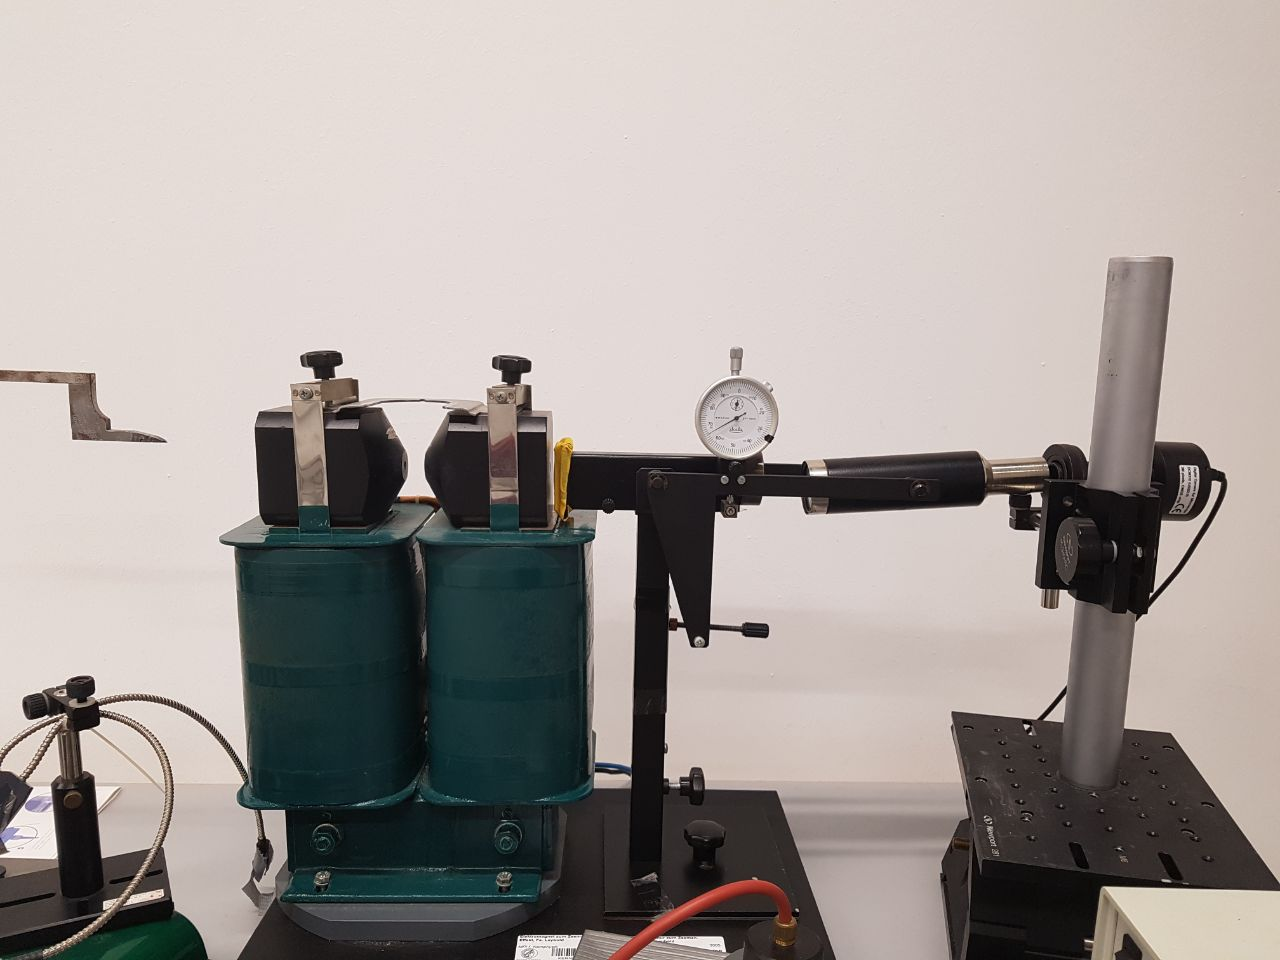
\includegraphics[width=0.6\linewidth]{img/IMG-20180102-WA0000.jpg}
                \caption{Versuchsaufbau, 1. Versuchsteil}
            \end{figure}
        \end{myframe}


    \subsection{2. Versuchsteil - Wellenlängenbestimmung}
        \begin{myframe}{\subsecname}
            \begin{itemize}
                \item Verwendung des Czerny - Turner Spektrometer um das Spektrum aufzunehmen
                \item Kalibrierung des Spektrometers mit Hilfe eines Referenzspektrums
                \item Bestimmung der Wellenlänge der roten Cadmium - Linie und einer unbekannten Linie
            \end{itemize}
        \end{myframe}

        \begin{myframe}{\subsecname}
            \begin{columns}
                \begin{column}{0.48\textwidth}
                    \begin{figure}
                        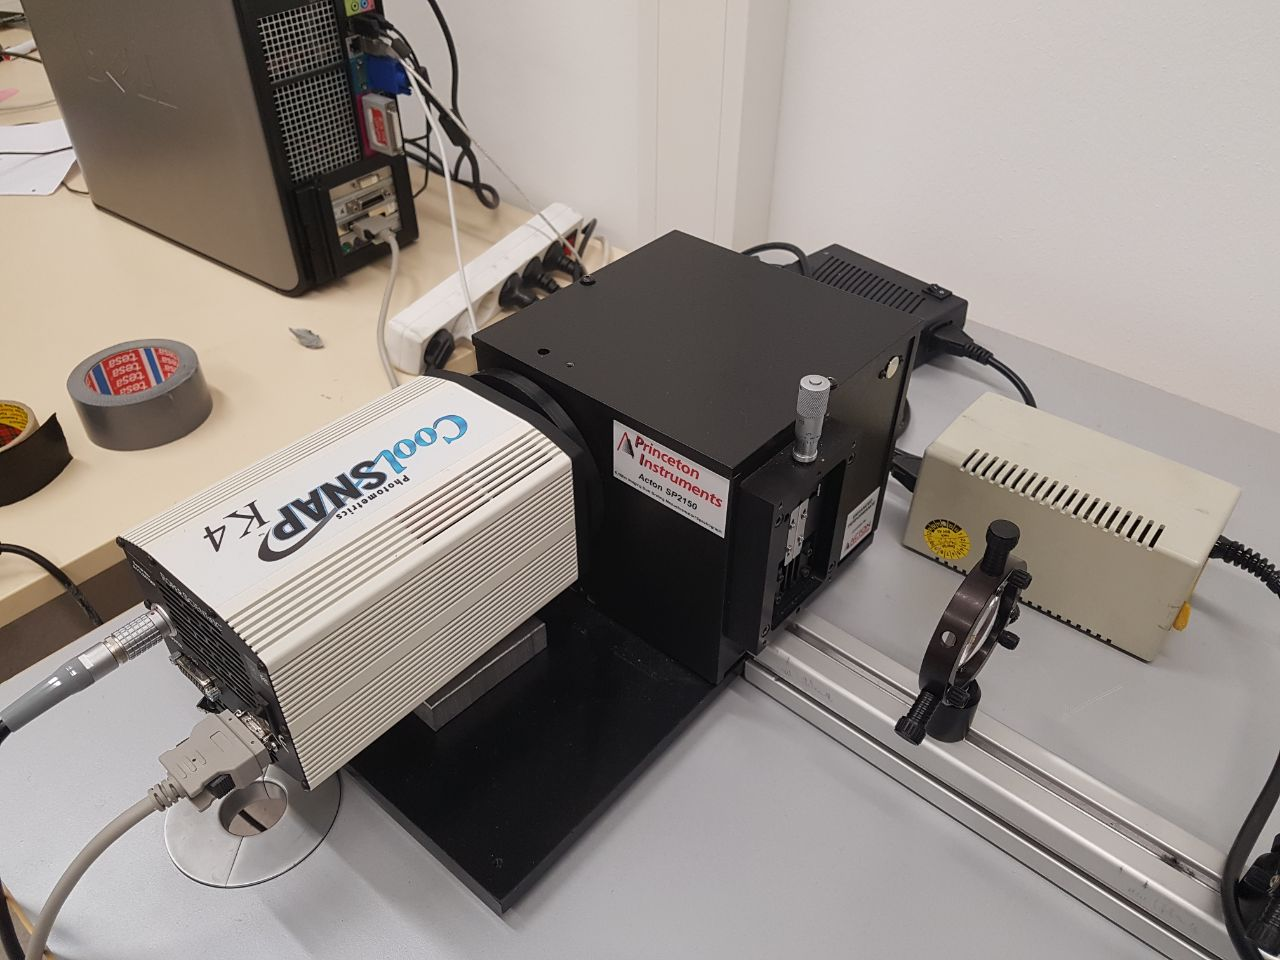
\includegraphics[width=0.8\linewidth]{img/IMG-20180102-WA0002.jpg}
                        \caption{Czerny - Turner Spektrometer}
                    \end{figure}
                \end{column}
                \begin{column}{0.48\textwidth}
                    \begin{figure}
                        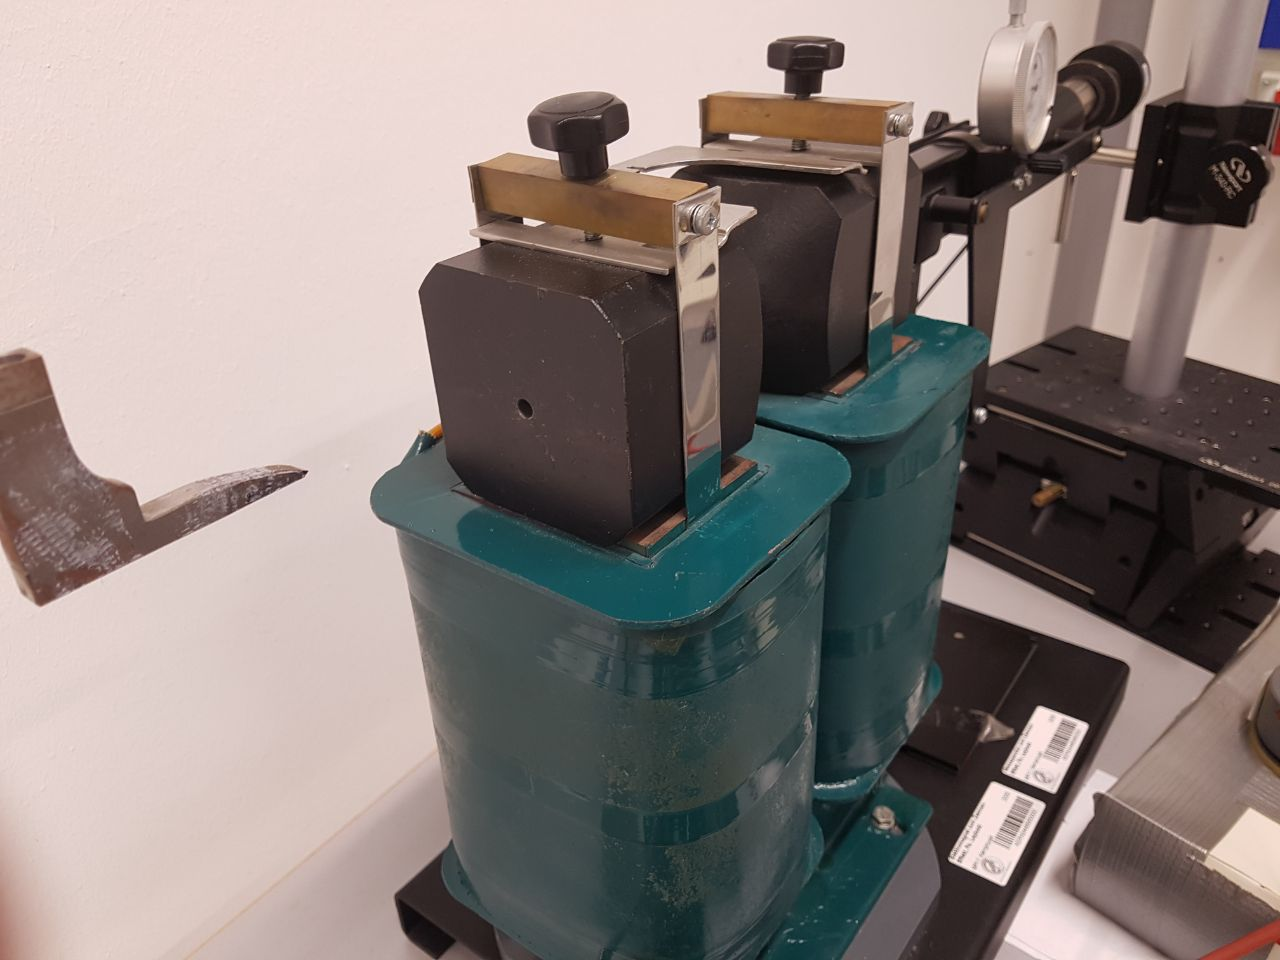
\includegraphics[width=0.8\linewidth]{img/IMG-20180102-WA0003.jpg}
                        \caption{Versuchsaufbau, 2. Versuchsteil}
                    \end{figure}
                \end{column}
            \end{columns}
        \end{myframe}

